\subsubsection{Влияние температуры на обилие \textit{Macoma~balthica}}
\textit{M.~balthica} --- вид, обладающий планктонной личинкой, при этом в условиях Белого моря от стадии велигера до метаморфоза и оседания проходит около месяца ($25 - 30$ суток) (\cite{Flyachinskaya_1999}). 
Известно, что общий личиночный пул формируется для достаточно крупных акваторий (\cite{Maximovich_Shilin_2012}). 
Поэтому расположенные на расстоянии около километра исследованные поселения, скорее всего, пополняются за счет общего личиночного пула, что влияет на синхронизацию динамики поселений. 
Однако данные по другим акваториям (\cite{Varfolomeeva_Naumov_2013}; А.В.~Герасимова, личное сообщение) показывают, что по крайней мере в $1998 - 1999$ году увеличение численности наблюдалось в разных районах Кандалакшского залива. 
Это дает основание предполагать влияние глобальных абиотических факторов, первым из которых может быть температура. 

Для проверки влияния температуры на динамику обилия \textit{M.~balthica} было проведено моделирование и использованием линейных моделей. 
Были использованы данные о температуре воздуха в Кандалакше. 
Полная модель включала в себя независимую переменную среднюю численность маком в данный год ($N_{t1}$) и независимые факторы: численность маком в предыдущий год ($N_{t}$), среднелетнюю температуру в предыдущий год ($T_{st}$) как отражение условий созревание гонад и формирования спата и среднезимнюю температуру в текущий год ($T_{wt1}$) как отражение критических условий первой зимы для сеголетков. 
Для выполнения условия о линейности зависимости, а также уменьшения воздействия влиятельных наблюдений в модели были использованы логарифмированные значения численности. 
В дальнейшем модель была редуцирована (полная и минимальная модели, ANOVA: $F = 0,43$; $p = 0,79$) и в минимальную модель в качестве факторов были включены $N_{t}$ и $T_{wt1}$. 
Характеристики полученной модели приведены в таблице~\ref{tab:model_koeff}. 
	\begin{table}[p]
	\caption{Характеристики модели зависимости обилия маком от их обилия в предыдущий год и зимней температуры.}
	\label{tab:model_koeff}
		\begin{tabularx}{\textwidth}{|X|X|X|X|X|}
			\hline
			факторы & Оценки  коэффициентов модели & Стандартная ошибка коэффициентов модели & $t$ & $P$ \\ \hline
			Свободный член & $1,96$ & $0,664$ & $2,96$ & $0,005$ \\ \hline
			$\ln(N_{t})$ & $0,60$ & $0,071$ & $8,44$ & $<0,0001$ \\ \hline
			$T_{wt1}$ & $-0,09$ & $0,036$ & $-2,50$ & $0,016$ \\ \hline
		\end{tabularx}
	\end{table}
Построенная модель удовлетворяла условиям применимости линейных моделей: отсутствия автокорреляций (критерий Дарбина-Уотсона: $1,71$; $p = 0,27$), нормальности распределения остатков (критерий Шапиро-Уилка: $W = 0,99$; $p = 0,86$) и гомогенности дисперсий (критерий Бройша-Пагана: $BP = 5,25$; $p-value = 0,15$). 
Таким образом, связь между обилием маком в текущий и в предыдущий год и зимней температурой описывается моделью вида: $\ln(N_{t1}) = 1,96 + 0,60 \times \ln(N_{t}) - 0,09 \times T_{wt1}$ ($F = 37,04$; $p < 0,0001$. $R^2 = 0,6$) (рис.~\ref{ris:model_temperature}).
	\begin{figure}[p]
		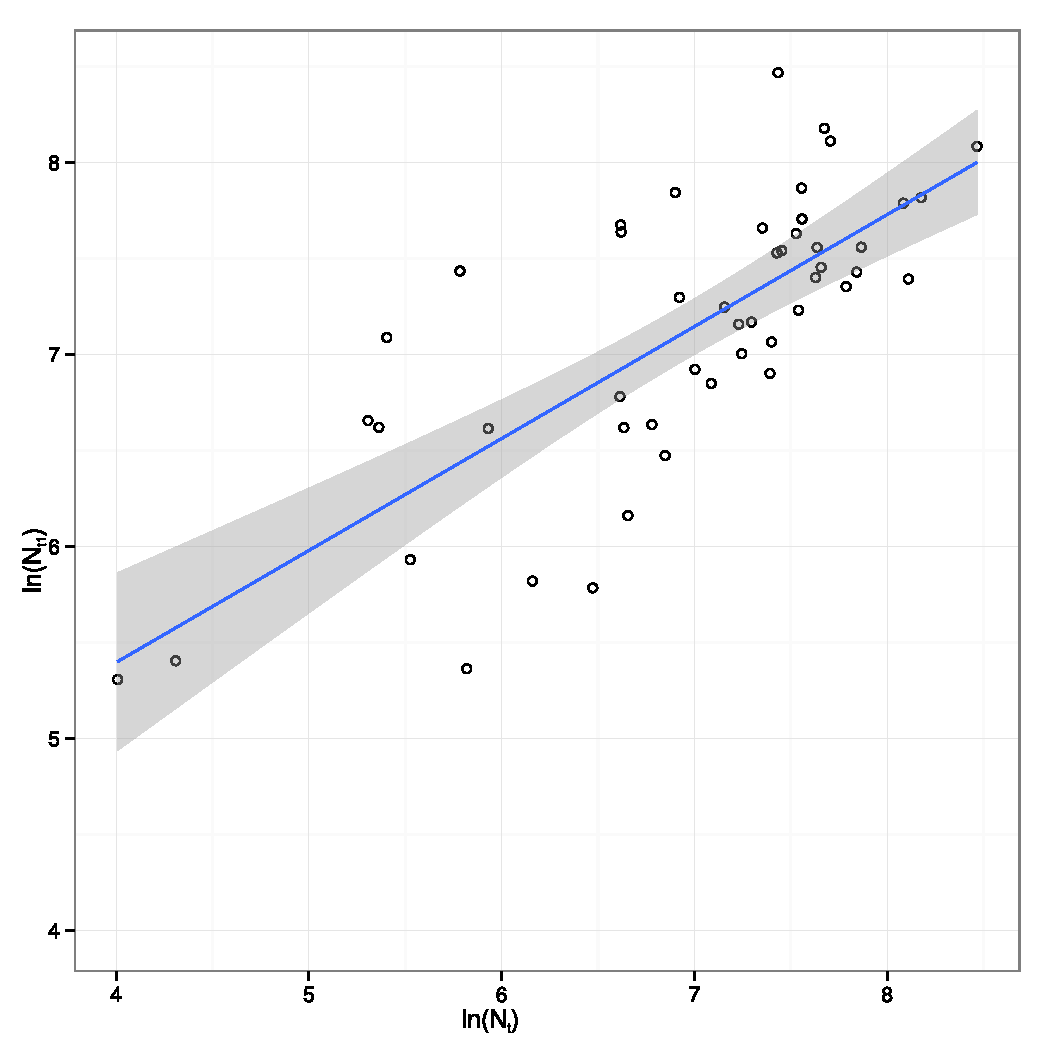
\includegraphics[height=0.4\textheight]{../article_Macoma_dynamic_White_sea/N_vs_temperature/lodNt_vs_logNt1_1.pdf}

		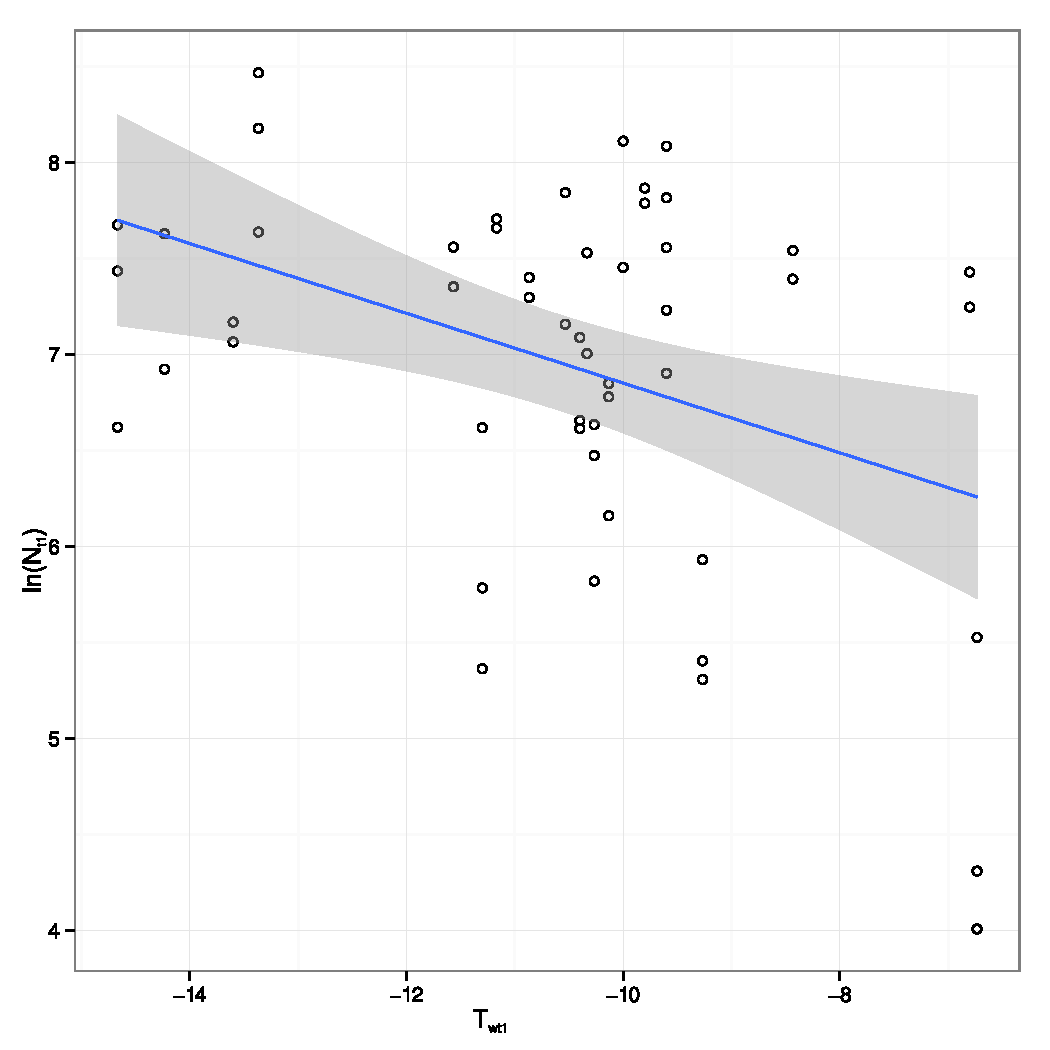
\includegraphics[height=0.4\textheight]{../article_Macoma_dynamic_White_sea/N_vs_temperature/Twt1_vs_logNt1_1.pdf}

	\caption{Зависимость численности  \textit{Macoma balthica} ($\ln(N_{t1})$) от численности в предыдущий год ($\ln(N_{t})$) и зимней температуры ($T_{wt1}$).}
	\label{ris:model_temperature}
	\footnotesize{Показаны линейная модель (синяя линия) и ее 95\% доверительный интервал (серая область).}
	\end{figure}

Полученные данные о влиянии зимней температуры противоречат нашей исходной гипотезе о том, что холодные зимы в Белом море критичны для маком. 
Результаты моделирования позволяют говорить о том, что обилие маком увеличивается после более холодных зим и уменьшается после относительно теплых (рис.~\ref{ris:model_temperature}). 
Данный результат хорошо согласуется с результатами полученными Бьёкема с соавторами (\cite{Beukema_et_al_1998, Beukema_et_al_2009}) для Ваттового моря. 

Для данной акватории было показано, что одним из ключевых факторов, влияющих на пополнение поселений \textit{M.~balthica}, является температура в зимний период. 
Пополнение после суровых зим было больше, чем после мягких. 
Было предложено два механизма, зависимые от зимней температуры: 
1. количество яиц маком, выметанных в апреле больше после холодной зимы, поскольку при низкой температуре меньше уровень обмена, а, значит, меньше потери веса за зиму, и больше энергии остается на продукцию. 
2. Биомасса \textit{Crangon crangon}, одного из важных хищников для маком, была значительно выше после холодных зим. 
При проверке обеих гипотез, было показано, что второй механизм влияет значительно сильнее (\cite{Beukema_et_al_1998, Beukema_Dekker_2014, Dekker_Beukema_2014}). 

В настоящее время у нас нет прямых данных, позволяющих говорить о механизмах влияния температуры на \textit{M.~balthica} в Белом море. 
Проведение аналогий с Ваттовым морем затруднено, поскольку считается, что роль хищников снижается в более полярных сообществах (\cite{Pianka_1966, Freestone_et_al_2011}). 
Возможно, уменьшение обилия маком после теплых зим связано с тем, что при более теплых зимах ледостав менее стабилен, и литораль во время отлива оказывается напрямую подвержена воздействию отрицательных температур воздуха, в то время как в холодные зимы стабильный ледовый покров создает изолирующий слой, и колебания температуры подо льдом оказываются значительно ниже (\cite{Kuznecov_1960}).

\afterpage{\clearpage}
